\chapter{Experimental Evaluation}\label{sec:eval}
To understand the practical performance of the proposed algorithms \textit{pSPIDER}, \textit{pBINDER} and \textit{SPIND} we use the known algorithms \textit{SPIDER} and \textit{BINDER} with their existing implementations. We will review the data sets utilized (Section \ref{subsec:datasets}) and present the execution times for all data sets across the different algorithms (Section \ref{subsec:runtime}). We will also discuss the impact of hyperparameter choices (Section \ref{subsec:hyperparameters}), the probabilistic filter (Section \ref{subsec:filter_res}), and finally examine pINDs in real-world data (Section \ref{subsec:real_pINDs}).

\chapter{Datasets}
To understand the performance of the proposed algorithms it is crucial to perform testing on a variety of data sets. For this purpose we will gather some real word data sets. Further we will create synthetic data sets that aim on edge cases to see if the performance is strongly dependent on structural assumptions.

\section{Real World Data Sets}
There are many sources for csv or tsv files online. I have decided to gather data from the US Government\footnote{\href{https://data.gov}{data.gov}}, the European Union\footnote{\href{https://data.europe.eu}{data.europe.eu}}, Kaggle\footnote{\href{https://kaggle.com}{Kaggle.com}}, Musicbrainz\footnote{\href{https://musicbrainz.org/}{musicbrainz.org}}, and Eurostat\footnote{\href{https://musicbrainz.org/}{ec.europa.eu}}. Further data set sources may be added. Related research papers sometimes discuss the origin of the used data, do not discuss the structure of the data they use \cite{papenbrock2017data,bauckmann2006efficiently, dursch2019inclusion, rostin2009machine}. In order to understand the resulting algorithm performance, we believe it is crucial to examine the data which is tested against. In this section we will discuss the data used and later try to understand why an algorithms performance may vary over different test sets.

\section{Synthetic Data Sets}
To evaluate the proposed algorithms under detailed aspects, we will generate synthetic data sets. The strategies and claims are based on \cite{jordon2022synthetic} synthetic data can be defined as \textit{data that has been generated using a purpose-built mathematical model or algorithm, with the aim of solving a (set of) data science task(s).} While we will not try to train a model with the synthetic data, it is still of great use for us, since we have absolute knowledge about the underlying structures. The decision is based on the fact that there is a lot of real word data available, since open data is a growing market which expected to grow even further \cite{EUopenData}. Synthetic data on the other hand enables us to evaluate the algorithm performances on edge cases, which we may not be able to find in the selection of real world data sets. \\

\noindent To test certain edge cases of the proposed algorithms, we will construct various edge case data sets. The \textit{SameSame} dataset consists of 32 attributes and 250.000 records. Each attribute carries the numbers 1 to 250.000 in the natural order. This means every attribute is a (partial) inclusion dependency of every other attribute. The same obviously also holds for combinations of columns. We will now calculate the expected number if (p)INDs in each layer. Since all candidates are perfect matches, the chosen threshold $\rho$ will not influence the number of pINDs. Table % TODO add ref
shows the number of candidates/pINDs for the \textit{SameSame} dateset.
% TODO calculate INDs
The edge case to test here is, how well the algorithm can understand equality relations and prune the candidate space. While this may seem like an unlikely edge case we will also investigate how often this happens in real world data sets. \\
% write about real world structures

\noindent Another source of synthetic data will be the TPC (Transaction Processing Performance Council) Benchmarks \footnote{\href{https://www.tpc.org/}{tpc.org}}. The TPC Benchmarks are a set of standardized and vendor-neutral performance benchmarks used to evaluate the processing and database capabilities of different systems. These benchmarks are designed to model various types of workloads. The TPC-E benchmark, for example, models a brokerage firm with customers who generate transactions related to trades, account inquiries, and market research, while the TPC-C benchmark is intended to model a medium complexity online transaction processing workload, patterned after an order-entry system with skewed access within individual data types/relations. Using scaling factors, a user can define the size of the synthetic database themselves. This enables us to examine the algorithm performances in a very controllable setting.



\section{Filter Evaluation} \label{subsec:filter_res}
We would like to understand the effect of using a probabilistic filter. In Section \ref{subsec:prob_filter} we discuss two versions. A filter which is built once after unary discovery and a filter which is rebuild on every nary layer. In Figure \ref{fig:filter} we find the execution times of all datasets, expect \textbf{WebTables} since we only search for unarys in that case. The graphic shows the difference in runtime when using the bloom filter by constructing it once during unary discovery (\textit{Once}), using and refining the filter at every level (\textit{Refine}) and not using a probabilistic filter at all. Not using a filter builds the baseline execution time, while the other two modes are displayed with their relative runtime to that baseline.

We find that the results vary substantially when viewing the different datasets. This observation supports the notion that we succeeded in finding a range of datasets which are structurally different from each other. Notably, \textit{TPC-H 1} and \textit{UniProt} performed better without a probabilistic filter. For \textit{UniProt} we find that the filter does decrease the execution time since the data set exclusively produces symmetrically INDs. For \textit{TPC-H 1}, we observe that the number of n-ary candidates is so limited that the time spent on construction exceeds the computational savings achieved. Employing either a filter build once or a refined filter yields nearly identical execution times, which are generally slightly quicker than not using a filter at all. Given that a refined filter can reduce some read and write operations, we opt for this version to reduce the disk workload.

\begin{figure}[t!]
    \centering
    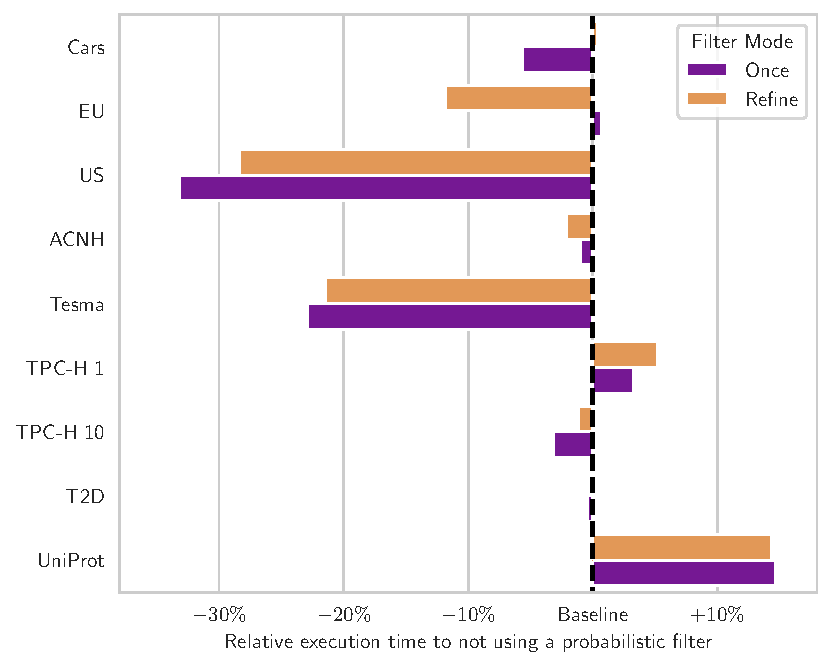
\includegraphics[width=.6\textwidth]{figures/filter_results.pdf}
    \caption{Changes in execution time when using a (refined) probabilistic filter for nary IND discovery.}
    \label{fig:filter}
\end{figure}

\section{Real World pINDs} \label{subsec:real_pINDs}
Real-world datasets exhibit a considerable amount of pINDs, even when the identification threshold for such relationships is set to a high value (e.g., $\rho = 0.99$). Some of these pINDs are logical and significant, indicating underlying patterns or connections within the data. For example, date columns may not be perfectly contained within each other due to differences in update frequencies across data sets (found in the \textit{EU} data set). However, pINDs also occur purely by chance, without any substantial relevance. Consequently, human expertise is essential to evaluate whether a discovered pIND is truly useful, as automated detection alone cannot adequately distinguish between meaningful dependencies and coincidental ones.